\documentclass[10pt,svgnames,fragile]{beamer}
\usepackage[utf8]{inputenc}
\usepackage{lmodern}
\usepackage[T1]{fontenc}
\usepackage{graphicx}
\usepackage{xcolor}
\usepackage{amsmath}
\usepackage{amssymb}
\usepackage{amsthm}
\usepackage{qtree}
\usepackage{tikz}
\usepackage{hyperref}
\usepackage{xcolor}
\usepackage{tikz}
\usepackage{amsmath, amssymb}
\usetikzlibrary{shapes,arrows,positioning}
\usepackage{amsmath, amssymb}
\usepackage{tcolorbox}
\usetheme{Madrid}



%% Show outline at the beginning of each section
\AtBeginSection[]{\begin{frame}\frametitle{Outline}\tableofcontents[currentsection,hideothersubsections]\end{frame}}

\usetheme{CambridgeUS}
\usecolortheme{dolphin}
\setbeamertemplate{navigation symbols}{}

\title{Tree Automata (UMC 205)}
% \subtitle{UMC 205 Seminar}
\author{Himesh(23775), Kuldeep(23684), Shobhnik(23697) }
\date{5th April 2025}

\begin{document}

\begin{frame}
  \titlepage
\end{frame}

\begin{frame}{Outline}
  \tableofcontents
\end{frame}

\section{Introduction}

\begin{frame}{From Strings to Trees}
  \begin{itemize}
    \item Most automata models work on strings over finite alphabets
    \item But many problems have inputs more structured than strings
    \item Trees arise in a variety of contexts:
      \begin{itemize}
        \item Arithmetic expressions
        \item Logical formulas
        \item Parse trees of grammars
        \item HTML documents
      \end{itemize}
    \item Tree automata provide a natural way to process such structured inputs
  \end{itemize}
\end{frame}

\begin{frame}{Examples of Tree Structures}
  \begin{columns}
    \begin{column}{0.33\textwidth}
      \begin{center}
        \begin{tikzpicture}[level distance=0.8cm, 
                   level 1/.style={sibling distance=2cm},
                   level 2/.style={sibling distance=1cm}]
          \node {$\sqrt{}$}
            child { node {$\cdot$}
              child { node {$x$} }
              child { node {$+$} 
                child { node {$y$} }
                child { node {$3$} }
              }
            };
        \end{tikzpicture}
        
        Expression $\sqrt{x \cdot (y + 3)}$
      \end{center}
    \end{column}
    \begin{column}{0.33\textwidth}
      \begin{center}
        \begin{tikzpicture}[level distance=0.8cm, 
                   level 1/.style={sibling distance=1.5cm},
                   level 2/.style={sibling distance=1cm}]
          \node {$\land$}
            child { node {$x$} }
            child { node {$\lnot$}
              child { node {$\lor$} 
                child { node {$y$} }
                child { node {$z$} }
              }
            };
        \end{tikzpicture}
        
        Formula $x \land \lnot(y \lor z)$
      \end{center}
    \end{column}
    \begin{column}{0.33\textwidth}
      \begin{center}
        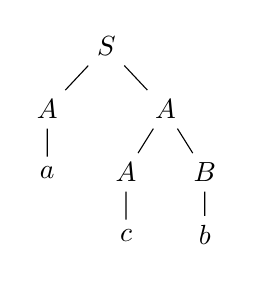
\begin{tikzpicture}[level distance=0.8cm, 
                   level 1/.style={sibling distance=1.5cm},
                   level 2/.style={sibling distance=1cm}]
          \node {$S$}
            child { node {$A$} 
              child { node {$a$} }
            }
            child { node {$A$}
              child { node {$A$} 
                child { node {$c$} }
              }
              child { node {$B$} 
                child { node {$b$} }
              }
            };
        \end{tikzpicture}
        
        Parse tree of grammar\\
        $S \rightarrow AA$\\
        $A \rightarrow a | c | AB$\\
        $B \rightarrow b$ \\
        derivation tree for "acb"
      \end{center}
    \end{column}
  \end{columns}
\end{frame}

\section{Tree Domains and Labeled Trees}

\begin{frame}{Tree Domains and Labeled Trees}
  \begin{definition}
    An $n$-ary tree domain, $\text{dom}_t$, is a prefix closed subset of $\{0,1,2,\ldots,n-1\}^*$ such that if $ui \in \text{dom}_t$ then $uj \in \text{dom}_t$ for every $j < i$.
  \end{definition}
  
  \begin{definition}
    A $\Gamma$-labeled $n$-ary tree is a pair $t = (\text{dom}_t, \text{val}_t)$, where $\text{dom}_t$ is an $n$-ary tree domain and $\text{val}_t : \text{dom}_t \rightarrow \Gamma$ is a labeling function.
  \end{definition}
  
\end{frame}
\newpage
\vspace{20pt}

\begin{frame}{Example}
    For the tree representing $\sqrt{x \cdot (y + 3)}$:
    \begin{center}
    \begin{minipage}{0.5\textwidth}
    
    \begin{itemize}
      \item Root is named $\varepsilon$ (labeled $\sqrt{}$)
      \item Its child is $0$ (labeled $\cdot$)
      \item Other vertices are $00$ (labeled $x$), $01$ (labeled $+$)
      \item And $010$ (labeled $y$), $011$ (labeled $3$)
    \end{itemize}
  % \end{block}
\end{minipage}
\hfill
\begin{minipage}{0.4\textwidth}
        \begin{center}
        \begin{tikzpicture}[level distance=0.8cm, 
                   level 1/.style={sibling distance=2cm},
                   level 2/.style={sibling distance=1cm}]
          \node {$\sqrt{}$}
            child { node {$\cdot$}
              child { node {$x$} }
              child { node {$+$} 
                child { node {$y$} }
                child { node {$3$} }
              }
            };
        \end{tikzpicture}
        
        Expression $\sqrt{x \cdot (y + 3)}$
      \end{center}
\end{minipage}
\end{center}
\end{frame}





\begin{frame}{Tree Operations}
  \begin{block}{Building Trees}
    Given $\Gamma$-labeled trees $t_0 = (\text{dom}_{t_0}, \text{val}_{t_0})$ and $t_1 = (\text{dom}_{t_1}, \text{val}_{t_1})$, and $A \in \Gamma$, the tree $A(t_0, t_1)$ is given by $t = (\text{dom}_t, \text{val}_t)$ where:
    \begin{align*}
      \text{dom}_t &= \{\varepsilon\} \cup \{0u | u \in \text{dom}_{t_0}\} \cup \{1u | u \in \text{dom}_{t_1}\} \\
      \text{val}_t(u) &= 
      \begin{cases}
        A & \text{if } u = \varepsilon \\
        \text{val}_{t_0}(v) & \text{if } u = 0v \\
        \text{val}_{t_1}(v) & \text{if } u = 1v
      \end{cases}
    \end{align*}
  \end{block}
  
  \pause
  
  \begin{block}{Subtrees}
    Given a $\Gamma$-labeled tree $t = (\text{dom}_t, \text{val}_t)$ and vertex/position $p \in \text{dom}_t$, subtree rooted at position $p$ is the tree $t|_p = (\text{dom}_{t|_p}, \text{val}_{t|_p})$ given by:
    \begin{align*}
      \text{dom}_{t|_p} &= \{u | pu \in \text{dom}_t\} \\
      \text{val}_{t|_p}(u) &= \text{val}_t(pu)
    \end{align*}
  \end{block}
\end{frame}

\section{Deterministic Tree Automata}

\begin{frame}{Deterministic Tree Automata (DTA)}
  \begin{definition}
    A deterministic tree automaton (DTA) on $\Sigma$-labeled $n$-ary trees is $M = (Q, \Sigma, \delta, F)$ where:
    \begin{itemize}
      \item $Q$ is a finite set of states
      \item $F \subseteq Q$ is a set of final/accepting states
      \item $\delta = \cup_{i=0}^{n} \delta_i$ is the transition function, where $\delta_i: Q^i \times \Sigma \to Q$
    \end{itemize}
  \end{definition}
  
  \pause
  
  \begin{block}{Run of a DTA}
    The run of a DTA $M = (Q, \Sigma, \delta, F)$ on a tree $t = (\text{dom}_t, \text{val}_t)$ is a $Q$-labeled tree $\rho = (\text{dom}_\rho, \text{val}_\rho)$ where $\text{dom}_\rho = \text{dom}_t$ and for any vertex $u \in \text{dom}_t$ with $i$ children:
    \begin{align*}
      \text{val}_\rho(u) = \delta_i(\text{val}_\rho(u0), \ldots \text{val}_\rho(u(i-1)), \text{val}_t(u))
    \end{align*}
  \end{block}
\end{frame}

\begin{frame}{Acceptance and Language}
  \begin{block}{Acceptance}
    A run $\rho = (\text{dom}_\rho, \text{val}_\rho)$ of $M$ on $t$ is accepting if $\text{val}_\rho(\varepsilon) \in F$.
    
    A tree $t$ is accepted by $M$ if $M$ has an accepting run on $t$.
  \end{block}
  
  \pause
  
  \begin{block}{Language}
    The language recognized by $M$ is the set of all $\Sigma$-labeled $n$-ary trees it accepts:
    \begin{align*}
      L(M) = \{t | M \text{ accepts } t\}
    \end{align*}
  \end{block}
  
  \pause
  
  \begin{definition}
    A set $A$ of $\Sigma$-labeled $n$-ary trees is regular if there is a DTA $M$ such that $A = L(M)$.
  \end{definition}
\end{frame}

\begin{frame}{Example: Boolean Expression Evaluator}
  \begin{block}{DTA for Boolean Expressions}
    Let $\Sigma = \{0, 1, \neg, \wedge, \vee\}$. Consider the DTA $M_p = (\{q_0, q_1, q_r\}, \Sigma, \delta, \{q_1\})$ where:
    \begin{align*}
      \delta_0(0) &= q_0 & \delta_0(1) &= q_1 \\
      \delta_1(q_0, \neg) &= q_1 & \delta_1(q_1, \neg) &= q_0 \\
    \end{align*}
    
    For $\wedge$:
    \begin{align*}
      \delta_2(q_i, q_j, \wedge) &= 
      \begin{cases}
        q_1 & \text{if } q_i = q_j = q_1 \\
        q_0 & \text{if } \{q_i, q_j\} \cap \{q_r\} = \emptyset \text{ and } \{q_i, q_j\} \cap \{q_0\} \neq \emptyset
      \end{cases}
    \end{align*}
    
    For $\vee$:
    \begin{align*}
      \delta_2(q_i, q_j, \vee) &= 
      \begin{cases}
        q_0 & \text{if } q_i = q_j = q_0 \\
        q_1 & \text{if } \{q_i, q_j\} \cap \{q_r\} = \emptyset \text{ and } \{q_i, q_j\} \cap \{q_1\} \neq \emptyset
      \end{cases}
    \end{align*}
    
    For all other cases, $M_p$ transitions to state $q_r$.
  \end{block}
\end{frame}

\begin{frame}{Example: Boolean Expression Evaluator}
  \begin{columns}
    \begin{column}{0.45\textwidth}
      \begin{center}
        \begin{tikzpicture}[level distance=0.8cm, 
                   level 1/.style={sibling distance=1.5cm},
                   level 2/.style={sibling distance=1.5cm},
                   level 3/.style={sibling distance=0.7cm}]
          \node {$\neg$}
            child { node {$\vee$}
              child { node {$\wedge$} 
                child { node {$0$} }
                child { node {$1$} }
              }
              child { node {$\wedge$} 
                child { node {$0$} }
                child { node {$0$} }
              }
            };
        \end{tikzpicture}
        
        Input tree $\neg((0 \wedge 1) \vee (0 \wedge 0))$
      \end{center}
    \end{column}
    \begin{column}{0.45\textwidth}
      \begin{center}
        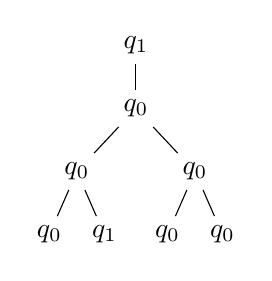
\begin{tikzpicture}[level distance=0.8cm, 
                   level 1/.style={sibling distance=1.5cm},
                   level 2/.style={sibling distance=1.5cm},
                   level 3/.style={sibling distance=0.7cm}]
          \node {$q_1$}
            child { node {$q_0$}
              child { node {$q_0$} 
                child { node {$q_0$} }
                child { node {$q_1$} }
              }
              child { node {$q_0$} 
                child { node {$q_0$} }
                child { node {$q_0$} }
              }
            };
        \end{tikzpicture}
        
        Run of DTA $M_p$ on the input
      \end{center}
    \end{column}
  \end{columns}
  
  \begin{itemize}
    \item Since the label of the root in the run is $q_1 \in F$, this input is accepted
    \item $L(M_p)$ = set of syntactically correct boolean expressions that evaluate to true
  \end{itemize}
\end{frame}

\begin{frame}{Example: Arithmetic Modulo 3}
  \begin{block}{DTA for Arithmetic Expressions}
    For $\Sigma = \{0, 1, 2, +, \cdot\}$. Consider the DTA $M_a = (\{q_0, q_1, q_2, q_r\}, \Sigma, \delta, \{q_0\})$ where:
    \begin{align*}
      \delta_0(0) &= q_0  \hspace{2cm} \delta_0(1) = q_1 & \hspace{2cm} \delta(2) = q_2 \\
      \delta_2(q_i, q_j, +) &= q_{(i+j) \bmod 3} & \text{if } \{q_i, q_j\} \cap \{q_r\} = \emptyset \\
      \delta_2(q_i, q_j, \cdot) &= q_{(i \cdot j) \bmod 3} & \text{if } \{q_i, q_j\} \cap \{q_r\} = \emptyset
    \end{align*}
    
    In all other cases not considered above, $\delta$ returns $q_r$.
  \end{block}
  
  \begin{itemize}
    \item Trees over $\Sigma$ represent arithmetic expressions
    \item If they are syntactically correct, $M_a$'s run will have root labeled $q_i$, where $i$ is the remainder when the value of the expression is divided by 3
    \item Since the final state is $q_0$, the automaton accepts expressions that evaluate to multiples of 3
  \end{itemize}
\end{frame}

\section{Nondeterministic Tree Automata}

\begin{frame}{Nondeterministic Tree Automata}
  \begin{definition}
    A nondeterministic tree automaton (NTA) on $\Sigma$-labeled $n$-ary trees is $M = (Q, \Sigma, \delta, F)$ where $Q$ is a finite set of states, $F \subseteq Q$ is a set of final/accepting states, and $\delta = \cup_{i=0}^{n} \delta_i$ is the transition function, where $\delta_i: Q^i \times \Sigma \to 2^Q$.
  \end{definition}
  
  \pause
  
  \begin{theorem}
    Let $A$ be a tree language recognized by an NTA. Then $A$ is regular.
  \end{theorem}
  \pause
  \begin{proof}[Proof Sketch]
    The standard subset construction extends to tree automata:
    \begin{itemize}
      \item Convert NTA $N = (Q, \Sigma, \delta, F)$ to DTA $D = (2^Q, \Sigma, \delta', F')$
      \item $F' = \{P \subseteq Q \mid P \cap F \neq \emptyset\}$
      \item $\delta'_0 = \delta_0$ and $\delta'_k(Q_1, Q_2, \ldots, Q_k, f) = \{q \mid \exists q_1, q_2, \ldots, q_k. q_i \in Q_i \text{ and } q \in \delta_k(q_1, q_2, \ldots, q_k, f)\}$
    \end{itemize}
  \end{proof}
\end{frame}

\section{Properties of Tree Automata}

\begin{frame}
    \begin{block}{Claim} Every finite set of trees is regular \end{block}
    \pause
    \begin{proof}
        Let $T = \{t_1,t_2...,t_n\}$ , be the set of finite number of trees \vspace{7pt}
        \begin{itemize}
        \begin{itemize}
            \item \textbf{States}: 
            \begin{itemize}
                \item Let $S = \{\text{all subtrees of } t_i \in T\}$ (finite set)
                \item $Q = S \cup \{q_{\text{sink}}\}$
            \end{itemize}
            
            \item \textbf{Accepting States}:
            \begin{itemize}
                \item $F = \{t_1, t_2, \ldots, t_n\} \subseteq Q$
            \end{itemize}
    
            
            \item \textbf{Transition Function $\delta$}:
            \begin{itemize}
                \item For node `$a$' with children in states $s_1, \ldots, s_k$:
                \[
                \delta( s_1, \ldots, s_k, a) = 
                \begin{cases}
                    s & \text{if } \exists s \in S \text{ matches subtree rooted at } \text{`}a\text{'} \\
                    q_{\text{sink}} & \text{otherwise}
                \end{cases}
                \]
            \end{itemize}
        \end{itemize}
    \end{itemize}
    \end{proof}
\end{frame}

\begin{frame}{DTA for Parse Trees}
    \begin{block}{Claim}
        The set of derivation trees/parse trees of a context-free grammar \( G = (N, T, P, S) \) is regular.
    \end{block}
    \pause
    \begin{proof}
        Take \( \Sigma = N \cup T \). The automaton recognizing the parse trees is:
        
        \begin{itemize}
            \item \textbf{States: } \( Q = T \cup N \cup \{*\} \)
            \item \textbf{Final States: } \( F = \{S\} \)
            \item \textbf{Transitions: } 
                \begin{itemize}
                    \item For \( i = 0 \): \( \delta_0(a) = a \) where \( a \in T \)
                    \item For \( i > 0 \): 
                    \( \delta_i(\alpha_1, \ldots, \alpha_i, X) = \begin{cases}
                        X & \text{if } X \to \alpha_1 \cdots \alpha_i \in P \\
                        * & \text{otherwise}
                    \end{cases} \)
                \end{itemize}
        \end{itemize}
    \end{proof}
\end{frame}

\begin{frame}{Non Regularity}

\textbf{Can you think of a tree language that is not regular ?}

\pause 

\begin{block}{Example Non-Regular Tree Languages}
    
    \begin{align*}
      L = \{A(t, t) \mid t \in T(\Sigma)\}
    \end{align*}
    where $T(\Sigma)$ is the collection of all full binary trees with leaves labeled by $b$ and internal vertices labeled by $A$. \vspace{6pt}
    
    \textbf{Proof by contradiction: } If $L$ is recognized by a DTA with finitely many states, then we can find two distinct trees $t_1 \neq t_2$ such that the DTA reaches the same state after reading either tree, which implies $A(t_1, t_2) \in L$, a contradiction.
  \end{block}
    
\end{frame}

\begin{frame}{Closed under Union}
    \begin{block}{Union}
        Let $L_1$ and $L_2$ be two recognizable tree languages and
$T_1 = (Q_1, \delta_1, F_1)$ and $T_2 = (Q_2, \delta_2, F_2)$ be the corresponding
tree automata. Then $L_1 \cup L_2$ is also a recognizable tree
language and is accepted by the automaton $T_1 \times T_2$
    \end{block}
    \pause
    \begin{block}{Construction}
        \begin{itemize}
            \item $Q = Q_1 \times Q_2$
            \item $\delta = \delta_1 \times \delta_2  $  i.e $\delta(t) : (Q_1 \times Q_2)^k \rightarrow Q_1 \times Q_2$ for $t \in \Sigma_k$
            \item $F = (F_1 \times Q_2) \cup (F_2 \times Q_1)$
        \end{itemize}
    \end{block}
\end{frame}

\begin{frame}{Closed under Complement}
    \begin{block}{Complement}
        Let L be a recognizable tree language and $T = (Q, \delta, F)$ be the
corresponding automaton over the alphabet $\Sigma$. Then the complement of L is also
a recognizable tree language and is accepted by the
automaton $T' = (Q, \delta, Q \textbackslash F)$
    \end{block}
\end{frame}

\begin{frame}{Closed under Intersection}
    \begin{block}{Intersection}
        Let $L_1$ and $L_2$ be two recognizable tree languages and
$T_1 = (Q_1, \delta_1, F_1)$ and $T_2 = (Q_2, \delta_2, F_2)$ be the corresponding
automata. Then $L_1 \cap L_2$ is also a recognizable tree language
and is accepted by the automaton$ T_1 \cap T_2$
    \end{block}
    \pause
    \begin{block}{Construction}
        \begin{itemize}
            \item $Q = Q_1 \times Q_2$
            \item $\delta = \delta_1 \times \delta_2$
            \item $F = F_1 \times F_2 $
        \end{itemize}
    \end{block}
\end{frame}

\section{Decision Problems}

\begin{frame}{Decision Problems}
  \begin{theorem}
    Given an NTA $M = (Q, \Sigma, \delta, F)$ there is a algorithm to determine if $L(M) = \emptyset$.
  \end{theorem}
  
  \pause
  
  \begin{proof}[Proof Sketch]
    Inductively compute the set of states that can be reached on some input:
    \begin{align*}
      E_0 &= \{q \mid \exists a \in \Sigma \ \ \text{and} \ \ q \in \delta_0(a)\} \\
      E_i &= E_{i-1} \cup \bigcup_k \{q \mid \exists a \in \Sigma ,\exists \  q_0, \ldots q_{k-1} \in E_{i-1} ,  q \in \delta_k(q_0, q_1, \ldots q_{k-1}, a)\}
    \end{align*}
    
    Since $M$ has finitely many states, for some $\ell$ (at most $|Q|$), $E_\ell = E_{\ell+1} = \{q \mid \exists t. q \text{ is reached on } t\}$.
    Therefore, $L(M) = \emptyset$ iff $E_\ell \cap F = \emptyset$.
  \end{proof}
    \pause 
    \begin{block}{Time Complexity : $O(|Q||\delta|)$}
    where $| \delta |$  is the number of transitions and $|Q|$ is the number of states.
    \end{block}
\end{frame}

\begin{frame}{Universality}
      \begin{corollary}
    Given a DTA $M$, there is a polynomial time algorithm to check if $L(M)$ contains all $\Sigma$-labeled trees.
  \end{corollary}
\end{frame}

\section{Applications}

\begin{frame}{Applications: Two-Player Games}
  \begin{block}{Game Setup}
      A game graph or arena is a $G = (Q_A, Q_B, E)$, where $Q_A$ and $Q_B$ are finite disjoint sets of vertices, and $E \subseteq (G_A \cup G_B) \times (G_A \cup G_B)$ is the edge relation with the property that every vertex has at least one outgoing edge.
  \end{block}
  \pause 
  \begin{block}{Game Rules}
      \begin{itemize}
          \item Initially the “token” is placed in some vertex
          \item In each move, the token is moved along an adjacent edge
          \item Who makes a move is decided by whose vertex it is
          
      \end{itemize}
  \end{block}
  \pause 
  \begin{block}{Winnig Criteria}
      Reachability to any final state $q \in F$ where $F \subseteq Q_A \cup Q_B$
  \end{block}
  \pause 
\vspace{4pt}
  \textbf{Can you figure out the initial states for which Bob has winning strategy?}
\end{frame}

\begin{frame}{Solution}

    \begin{center}
        \begin{figure}[h]
            \includegraphics[width=1\linewidth]{WhatsApp Image 2025-04-04 at 7.27.24 PM.jpeg}
            \label{fig:enter-label}
        \end{figure}
    \end{center}
\end{frame}

\begin{frame}{Solution}
\begin{tcolorbox}[colback=blue!5!white]
\textbf{Theorem.} The collection of winning strategies for Bob from position \( q \) is a regular tree language. The tree automaton recognizing this language can be effectively constructed.
\end{tcolorbox}

\pause
\vspace{2mm}

\textbf{Proof Sketch:}
\begin{itemize}
    \item \texttt{States:} Either game positions \( \overline{Q} \) (copy of \( Q_A \cup Q_B \)) or error state \( \ast \).
    \item \texttt{Transition Rules:}
    \begin{itemize}
        \item $\delta_0(q) = \bar{q}$ if $q\in F$
        \item $\delta_1(\bar{q_1},q) = \bar{q}$ if $(q,q_1)\in E$ and $q\in Q_B$
        \item $\delta_i(\overline{q_1}, \overline{q_2}, \dots, \overline{q_i}, q) = \overline{q}$ if $q \in Q_A $ and $ (q, q_1), \dots, (q, q_i)$ { are the only outgoing edges of } q
    \end{itemize}
\end{itemize}

\vspace{2mm}
\texttt{Formal Automaton Definition:}
\[
M = \left(\overline{Q} \cup \{\ast\},\; Q_A \cup Q_B,\; \delta,\; \{q\}\right)
\]
\end{frame}

\begin{frame}{Solution}
    \begin{block}{}
    \textbf{Theorem :} It can be decided whether Bob has a winning strategy from position $q$. Moreover if there is a winning strategy, it can be effectively constructed.
    \end{block}
    \pause 
    \begin{block}{}
    \textbf{Proof :} One can check the emptiness of the language associated with the DTA recognizing winning strategies from previous theorem.
    \end{block}
\end{frame}

\section{References}
\begin{frame}{Refrences}

\begin{itemize}
    \item {\hypersetup{urlcolor=red}\href{https://courses.grainger.illinois.edu/cs474/fa2021/fa2020Notes/TreeAutomata.pdf}{\textcolor{red}{Automata on Trees by Mahesh Viswanathan}}}
\end{itemize}
\end{frame}
\begin{frame}{}

\begin{center}
    \textbf{\Huge{Thank You!}}
\end{center}
    
\end{frame}

\end{document}
